\documentclass[laboratorio]{guia}

\def \practnum {7} 
\def \practica {Ondas ac\'usticas en un tubo}

\def \materia {Laboratorio de F\'\i sica II para Qu\'\i micos}
\def \periodo {2do. Cuatrimestre de 2015}
\def \catedra {Pablo Cobelli}
\def \website {http://materias.df.uba.ar/f2qa2015c2}
 
\usepackage{graphics}
\usepackage{amsmath}
\usepackage{amsfonts}
\usepackage{graphicx}
\usepackage{float}
\usepackage{wrapfig}
\usepackage{subfigure}
\usepackage{bm}
\usepackage{grffile}
\usepackage{color}
\usepackage{framed}
\usepackage[utf8]{inputenc}
\usepackage[T1]{fontenc}
\usepackage{lmodern}
\usepackage{circuitikz}
\usepackage[spanish]{babel}
\usepackage{babelbib}
\selectbiblanguage{spanish}

 

%----------------------------------------------------------
% Agrega al path de figuras el subdirectorio con el mismo
%     nombre que el archivo principal del proyecto
\graphicspath{{./\jobname/}}

%----------------------------------------------------------
% Definicion del entorno 'sabermas'
\makeatletter
\definecolor{shadecolor}{rgb}{0.89,0.91,0.94}
\newenvironment{sabermas}[1]{%
\vfill
\begin{shaded}
  \begin{center}
  {\textsection{Para saber m\'as}}
  \end{center}
  #1
\sf } 
{%
\end{shaded}%
}
\makeatother

%----------------------------------------------------------
% Definicion del entorno 'problema'
\newcounter{ContadorProblema}
\setcounter{ContadorProblema}{0}
\newcounter{TieneFiguraAsociada}
\setcounter{TieneFiguraAsociada}{0}
\newcounter{UbicacionFigura}
\setcounter{UbicacionFigura}{0}

\newenvironment{problema}[2][]
{%
    \ifx\relax#1\relax%
        \setcounter{TieneFiguraAsociada}{0}
        \else
        \setcounter{TieneFiguraAsociada}{1}
    \fi
    \def \archivofigura {#1}
    % 
    \refstepcounter{ContadorProblema}
    \noindent%
    \ifnum\value{TieneFiguraAsociada} < 1%
        {\sffamily \bfseries Problema \arabic{ContadorProblema}.}
        %{\sc {#1}}%
        \par\nobreak\par\nobreak%
        \medskip 
    \else
        % Va con figura; resta determinar de que lado.
        \ifnum\value{UbicacionFigura} < 1
            % Poner la figura del lado derecho
            \begin{minipage}{12.25cm}
            {\sffamily \bfseries Problema \arabic{ContadorProblema}.}
            %{\sc {#1}}%
            \par\nobreak\par\nobreak%
            \medskip 
        \else
            % Poner la figura del lado izquierdo
            \begin{minipage}{4.5cm}
                \centering
                \includegraphics[width=4.5cm]{\archivofigura}
                {\footnotesize {\sffamily Esquema asociado al 
                problema \arabic{ContadorProblema}}.}
            \end{minipage}\hfill%
            \begin{minipage}{12.25cm}
                {\sffamily \bfseries Problema \arabic{ContadorProblema}.}
                %{\sc {#1}}%
                \par\nobreak\par\nobreak%
                \medskip 
        \fi
    \fi
}
{%
    \ifnum\value{TieneFiguraAsociada} < 1%
        % \par \bigskip \vskip 0.3cm
    \else
        % Va con figura; resta determinar de que lado.
        \ifnum\value{UbicacionFigura} < 1
            % Poner la figura del lado derecho
            \end{minipage}\hfill%
            \begin{minipage}{4.5cm}
                \centering
                \includegraphics[width=4.5cm]{\archivofigura}
                {\footnotesize {\sffamily Esquema asociado al 
                problema \arabic{ContadorProblema}}.}
            \end{minipage}
        \else
            % Poner la figura del lado izquierdo
            \end{minipage}%
        \fi
    \fi
    \setcounter{TieneFiguraAsociada}{0}
    \par \bigskip \vskip 0.3cm
    % Permutamos el valor de la ubicacion
    \ifnum\value{UbicacionFigura} < 1
        \setcounter{UbicacionFigura}{1}
    \else
        \setcounter{UbicacionFigura}{0}
    \fi
}

%----------------------------------------------------------
% Definicion/Redefinicion de estilos
\renewcommand{\vec}[1]{\ensuremath{\mathbf{#1}}}



\hyphenation{ coe-fi-cien-tes coe-fi-cien-te au-to-va-lor
              au-to-va-lo-res co-rres-pon-der pro-ble-ma 
              cual-quie-ra po-la-ri-za-cio-nes }

\graphicspath{{./Guia_08_Ondas_Acusticas/}}

\begin{document} 
\objetivo{%
    El objetivo de esta pr\'actica es realizar un estudio experimental de ondas
    ac\'usticas en tubos semicerrados; en el cu\'al se
    determinen experimentalmente las frecuencias de resonancia y la velocidad de
    propagaci\'on del sonido.
    \tematicas{ondas estacionarias, ondas ac\'usticas, modos normales,
frecuencias caracter\'\i sticas, velocidad de propagaci\'on del sonido en aire.}} 
\maketitle

\section{Consideraciones preliminares}

La Figura~\ref{fig:1} muestra un esquema del dispositivo experimental propuesto
para el desarrollo de esta experiencia. Se dispone de un emisor ac\'ustico
(parlante) conectado a un generador de funciones capaz de emitir sonidos puros,
es decir, de una frecuencia bien definida. Asimismo, dicha frecuencia puede
variarse en un amplio rango de valores dentro del espectro audible. Tambi\'en
se cuenta con detectores de sonido (micr\'ofonos) conectados a osciloscopios
(o, en su defecto, a sistemas de adquisici\'on de datos asistidos por
computadora). 

\section{Desarrollo de la experiencia}

\subsection{Frecuencias de resonancia}

Usando un tubo semicerrado, comience por medir cuidadosamente las dimensiones
del tubo; su longitud $L$ y di\'ametro interno $d$. Para determinar sin
ambig\"uedad las frecuencias de resonancia asociadas a la presencia del tubo,
coloque el emisor y el receptor enfrentados, justo en el borde abierto del
tubo, seg\'un se muestra esquem\'aticamente en la Figura~\ref{fig:1}. Trate de
ubicar las frecuencias de resonancia, variando la frecuencia del generador de
funciones que alimenta el emisor. Preste particular atenci\'on a que la
amplitud del generador de funciones permanezca constante, lo cual se puede
lograr monitoreando la amplitud de la se\~nal de entrada al emisor. Las
resonancias se manifiestan por un pronunciado aumento de la amplitud de la
se\~nal de salida del receptor. En otras palabras, a las frecuencias de
resonancia, para una dada amplitud de la excitaci\'on del emisor, la respuesta
del receptor (su amplitud) tiene un m\'aximo relativo (dentro de un dado
intervalo de frecuencia).


\begin{figure}[t!]
    \centering
    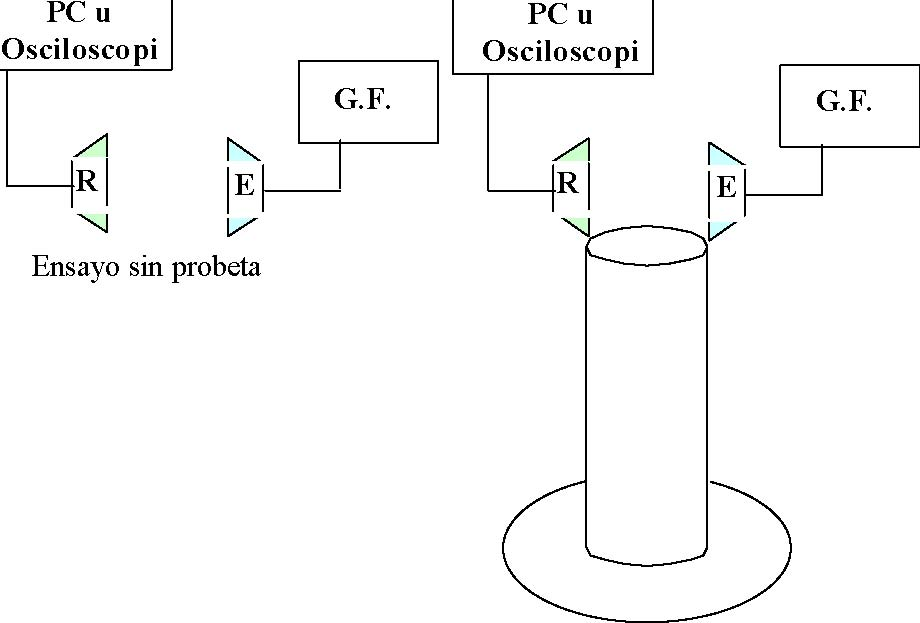
\includegraphics[width=8.5cm]{LG08--000.png}
    \caption{Esquema del dispositivo experimental para estudiar los modos de
    oscilaci\'on en un tubo.}
    \label{fig:1}
\end{figure}




En estas condiciones:
\begin{itemize}
    \item Determine por lo menos las primeras 5 resonancias en cada caso.
        Grafique la amplitud del receptor en funci\'on de la frecuencia
        aplicada. Para este estudio, intente mantener fija la geometr\'\i a del
        sistema (tubo, emisor, receptor, etc.) mientras var\'\i a la frecuencia
        de operaci\'on.
    \item Para verificar que las resonancias encontradas efectivamente est\'an
        asociadas al tubo y no a caracter\'\i sticas particulares del sistema
        emisor-receptor, retire el tubo y repita el estudio anterior, midiendo
        a las mismas frecuencias. Grafique luego la amplitud del receptor en
        funci\'on de la frecuencia aplicada, de ser posible sobre el mismo
        gr\'afico anterior. ?`Qu\'e puede concluir de este estudio acerca del
        origen de dichas resonancias?
    \item Grafique las frecuencias de resonancia del tubo en funci\'on del
        orden $n$ de cada resonancia, es decir, el \'\i ndice que identifica su
        aparici\'on cuando se incrementa mon\'otonamente la frecuencia. Busque
        determinar la frecuencia fundamental (correspondiente a $n=0$) por
        debajo de la cual no se detectan otras resonancias.
\end{itemize}


\subsection{Dependencia con la longitud del tubo}

En esta segunda parte nos proponemos determinar la variaci\'on en la respuesta
del sistema cuando se modifica la longitud del tubo considerado. Para ello, la
propuesta consiste en repetir el mismo estudio precedente para -al menos- dos
longitudes distintas a la empleada en la primera parte.


En estas nuevas condiciones:
\begin{itemize}
    \item Grafique las frecuencias de resonancia $f_n$ del tubo en funci\'on
        del orden $n$ de cada resonancia.
    \item Grafique el producto $f_nL$ en funci\'on del orden $n$, para todos
        los casos estudiados.
    \item Suponiendo que en el tubo semicerrado caben exactamente $(2n+1)$
        cuartos de longitudes de onda, trate de dar cuenta de sus resultados
        experimentales.
    \item A partir del gr\'afico de $f_nL$ en funci\'on de $(2n+1)$ y el modelo
        sugerido en el inciso anterior, determine el valor de la velocidad del
        sonido en aire. ?`C\'omo se compara su resultado con los valores
        tabulados? Discuta y especule acerca de las posibles discrepancias
        entre uno y otro. 
    \item Una consecuencia de tener un di\'ametro finito en el tubo es que su
        longitud efectiva es mayor que su longitud geom\'etrica. Esto causa que
        el n\'umero $n$ de medias longitudes de onda que caben en dicha
        longitud efectiva $L_\text{ef}$ satisfaga
        \begin{equation*}
            L_\text{ef} = L + \alpha d = n \frac{\lambda_n}{2}.
        \end{equation*}
        ?`C\'omo afecta esta correcci\'on sus conclusiones respecto de la
        velocidad de propagaci\'on del sonido en aire? Tenga en cuenta que el valor de $\alpha$ es del
        orden de 0.4 para un tubo semicerrado, y del orden de 0.8 para uno
        abierto.
\end{itemize}

\subsection{Ancho espectral de las resonancias}

Determine, para las resonancias encontradas en la primera parte, sus
respectivos semianchos en el espacio de frecuencias. Estos se definen como las
distancias (en frecuencia) en las que la amplitud cae a la mitad de su valor en
resonancia.

\subsection{Estudio en funci\'on de la posici\'on del detector}

Para por lo menos 3 frecuencias de resonancia, estudie experimentalmente c\'omo
var\'\i an la amplitud y la fase en funci\'on de la posici\'on del detector en
el tubo. Grafique sus resultados. ?`Qu\'e puede concluir acerca de estos
resultados? ?`Est\'an de acuerdo con la teor\'\i a propuesta? ?`C\'omo es la
amplitud en los extremos del tubo? Concretamente: en los extremos abierto y
cerrado, ?`hay nodos o extremos de amplitud? Explique sus resultados con
argumentos f\'\i sicos.

\nocite{Alonso1998,Crawford1994}
\bibliographystyle{unsrt} 
\bibliography{Bibliografia}




\end{document}
